%modified version of Niklaus Messerli by Gian Guido Parenza and Hendrik Klug
%to be printed on A4 borderless with 2 pages on one side


\documentclass[9pt]{article}
\usepackage[utf8]{inputenc}
\usepackage{lastpage}
\usepackage{amsmath}
\usepackage{amssymb}
\usepackage{dsfont}
\usepackage{array}
\usepackage{fancyhdr}
\usepackage[table]{xcolor}
\usepackage{xspace}
\usepackage{graphicx}
\usepackage{float}
\usepackage{wrapfig}
\usepackage{titlesec}
\usepackage{wrapfig}
\usepackage{mhchem}
\usepackage{multicol}
\usepackage{color}

% no paragraph indentation
\setlength\parindent{0pt}
\setlength{\parskip}{0pt}
\setlength{\parsep}{0pt}
\setlength{\headsep}{0pt}
\setlength{\topskip}{0pt}
\setlength{\topmargin}{0pt}
\setlength{\topsep}{0pt}
\setlength{\partopsep}{0pt}

%\usepackage[a4paper, lmargin=0.3cm,rmargin=0.3cm,tmargin=0.5cm,bmargin=0.5cm]{geometry}
\usepackage[a4paper, lmargin=0.3cm,rmargin=0.3cm,tmargin=0.5cm,bmargin=0.1cm]{geometry}

\definecolor{lightgrey}{gray}{0.9}
\newcommand{\grey}[1]{\setlength{\fboxsep}{0pt}\colorbox{lightgrey}{#1}}

% reduce space after subsubsection title
%\titlespacing*{\subsubsection}{0pt}{3.25ex plus 0ex minus .2ex}{0.5ex plus 0ex}
\usepackage{titlesec}
\titlespacing{\section}{0pt}{*0}{*0}
\titlespacing{\subsection}{0pt}{*0}{*0}
\titlespacing{\subsubsection}{0pt}{*0}{6pt}

\titleformat{\subsubsection}[runin]{\normalfont\bfseries}{\thesubsubsection}{3pt}{}[:]


% for table formatting
\def\arraystretch{1.3}
\definecolor{lgrey}{rgb}{0.9,0.9,0.9}
\newcolumntype{L}[1]{>{\raggedright\let\newline\\\arraybackslash\hspace{0pt}}m{#1}}
\newcolumntype{C}[1]{>{\centering\let\newline\\\arraybackslash\hspace{0pt}}m{#1}}
\newcolumntype{R}[1]{>{\raggedleft\let\newline\\\arraybackslash\hspace{0pt}}m{#1}}

% page header, no footer
\pagestyle{fancy}
%\lhead{Formulary Biomedical Imaging}
\lhead{}
%\chead{\thepage\ of \pageref{LastPage}}
\chead{}
%\rhead{HS2018}
\rhead{}
\fancyfoot{}
\renewcommand{\headrulewidth}{0.4pt}
\setlength{\headheight}{0pt}
\setlength{\headsep}{15pt}

% shortcuts
\newcommand{\dif}{\mathrm{d}}
\newcommand{\del}{\partial}
\newcommand{\fcal}{\mathcal{F}}
\newcommand{\TODO}{\colorbox{lime}{TODOTODOTODO}}

% danger symbol
\newcommand*{\TakeFourierOrnament}[1]{{%
		\fontencoding{U}\fontfamily{futs}\selectfont\char#1}}
\newcommand*{\danger}{\TakeFourierOrnament{66}}


\begin{document}

\fontsize{9.2pt}{10pt}\selectfont


\begin{multicols}{2}
\section{Imaging General}
\subsection{Plane Waves}
\vspace{-1mm}
\grey{$f(\vec{r},t)=A_0\cdot e^{j(\vec{k}\cdot \vec{r}-\omega t + \phi)}$}
$\vec{k}$ points in the direction of the wave and is orthogonal to the wavefront. $k_x \Delta x+k_y \Delta y = 2\pi$, \grey{$\lambda = 2\pi |\vec{k}|^{-1}$}
\subsection{Resolution}
\subsubsection{Spatial Resolution}
%LSF: Line Spread Function, PSF: Point Spread Function, Resolution = FWHM\{PSF\}, \grey{MTF = $\fcal$\{PSF\}}: Modulation Transfer Function.

Image($\vec r$) = Object $\ast$ PSF $(\vec r) 
\Rightarrow$  \grey{$\fcal \{\mathrm{Im}\}(\vec k) = \fcal \{\mathrm{Ob}\}(\vec k) \cdot \mathrm{MTF}(\vec k)$}

MTF describes attenuation of different spatial frequencies. Ideally constant ($\Leftrightarrow \mathrm{PSF} = \delta$), in reality Gaussian. \grey{SNR= Image intensity/std(intensity)} 

\subsubsection{Contrast}
\grey{$C =( I - I_\mathrm{background}) / I_\mathrm{background}$}. 

Scattering reduces contrast:
$C^\mathrm{sc} = \frac{(I + I_\mathrm{sc}) - (I_\mathrm{bg} + I_\mathrm{sc})}{I_\mathrm{bg} + I_\mathrm{sc}} = C \frac{1}{1 + I_\mathrm{sc}/I_\mathrm{bg}}$. 

Contrast in CT context: $C \propto (\mu_1 - \mu_2) d$

\subsubsection{Partial Volume Effect}
Happens because of insufficient \# of pixels covering the object, i.e. object smaller than 2$\times$FWHM resolution. $\Rightarrow$ underestimation of signal. Must not draw boundary of ROI too close to a tissue border.

\subsection{Fourier}
\vspace{-2mm}
Gauss $\leftrightarrow$ Gauss: $\sqrt{\frac{2\sigma^2}{\pi}} e^{-\sigma^2t^2/2} \leftrightarrow e^{-\omega^2/2\sigma^2}$

Const. $\leftrightarrow$ Dirac Delta; White Noise $\leftrightarrow$ White Noise

Comb $\leftrightarrow$ Comb: $\sum_n \delta(t - n\Delta t) \leftrightarrow \sum_n \delta(\omega - n \Delta \omega), \Delta\omega = 2\pi/\Delta t$

Exp $\leftrightarrow$ Lorentz: $e^{-|t|/T_2} \leftrightarrow \frac{2R_2}{(\omega^2 + R_2^2)}$

Sinc $\leftrightarrow$ Rectangle: $2\omega_c \mathrm{sinc}(\omega_c t) \leftrightarrow \chi_{[-\omega_c, \omega_c]}(\omega)$

\subsubsection{Projection Slice Theorem} FT of projection of 2D object is equal to slice through origin at same angle in 2D FT of whole object.

\subsection{Linear Shift Invariant Systems}
Different features should be imaged independently $\rightarrow$ Linear ($S[\alpha f_1 + f_2] = \alpha S[f_1] + S[f_2]$). Depiction of a feature should not depend of position $\rightarrow$ Shift Invariant. Complex exponentials (plane waves) are eigenfunctions $S[f] = S[f](0,0) \cdot f$ for $f(x,y) = e^{i(k_xx + k_yy)}$, where the eigenvalue is the transfer function $H(k_x,k_y)$.
\subsubsection{Fourier of LSI}
$\fcal\{S[f]\} = H(k_x,k_y) \cdot \fcal\{f\}(k_x,k_y) \Rightarrow S[f] = \fcal^{-1}\{H\} \ast f \Rightarrow $ \grey{$\mathrm{PSF} = \fcal^{-1}\{H\}$}

\subsection{Sampling Theorem}
\vspace{-1mm}
To prevent overlapping aliases: $\frac{2\pi}{\Delta x} > \mathrm{BW} \Leftrightarrow$ \grey{$\Delta x < \frac{2\pi}{\mathrm{BW}}= \frac{1}{2f_{max}}$}. For sampling k-space: \grey{$\Delta k < \frac{2\pi}{\mathrm{FOV}}$}
$\implies$ sampling range $\leftrightarrow$ resolution \\
\vspace{-5mm}
\subsection{Noise}
\textbf{Gaussian}: when many independent mechanisms superimpose $P_n(\eta)=\frac{1}{\sqrt{2\pi \sigma^2}}e^{-\frac{\eta ^2}{2\sigma ^2}}$, \textbf{Poisson}: when noise is related to discrete events $P_n(N)=\frac{\sigma ^{2N}}{N!}e^{-\sigma ^2}$, \textbf{SNR}: $\frac{|S[f](x,y)|}{\sigma_n}$
\section{X-Ray}
\subsection{Generation}
\begin{wrapfigure}[9]{l}{3cm}
	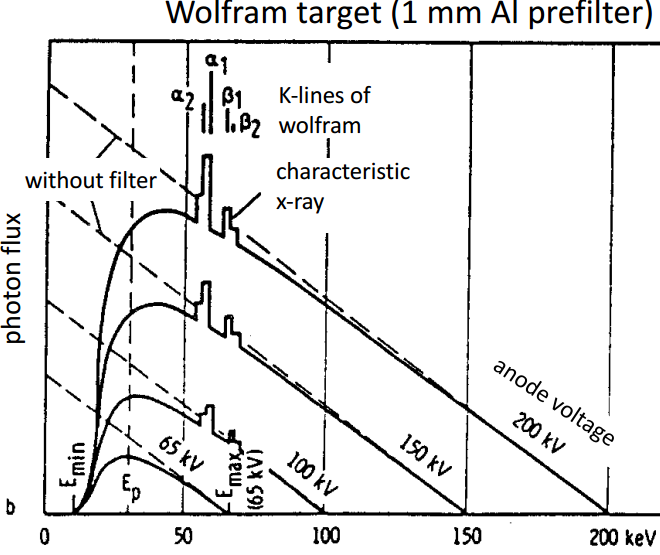
\includegraphics[width=3cm]{xrayspec.PNG}
\end{wrapfigure}
\vspace{-5mm}
$\lambda$ = 10pm - 10nm
\subsubsection{Bremsstrahlung}
Fast electron is deflected and slowed by nucleus, accelerated charge emits photon. Continuous spectrum. Interaction depends on $Z$ of nucleus and $E_e$. $E_{\gamma,max} = E_e$
\subsubsection{Characteristic Radiation}
Electron ejects K-shell e${}^-$ ($E_e > E_{binding,K}$), hole is refilled by L-shell or M-shell e${}^-$. Discrete energy peaks $E_\gamma = \hbar \omega = E_{binding,K}-E_{binding,L}$

\subsubsection{Heat Production}
Power absorption: \grey{$\alpha = \frac{P_{absorbed}}{P_{incident}}$}, Stefan-Boltzmann law: \grey{$W = \sigma(T^4 - T^4_{env})$} ($\sigma = 5.7\mathrm{e-}12 \mathrm{W\over cm^2\,K^4}$), Wien's displacement law: \grey{$\lambda_{peak} = \frac{b}{T}$} ($b=2.9\mathrm{e-}3$mK)

\subsection{Attenuation}
= Absorption + Scatter = Photoeffect + Compton Scattering
\subsubsection{Photoeffect} 
Is what provides contrast. $\gamma$ is fully absorbed, knocking e${}^-$ out of shell $\Rightarrow$ ionizing! Hole refilled $\Rightarrow$ low keV characteristic X-ray. Probability: \grey{$P_\mathrm{pe} \propto \rho \frac{Z_{\mathrm{eff}}^3}{E\gamma^3}$} with tissue density $\rho$ and $Z_\mathrm{eff}=$ 7.4(tissue), 6.9(lipid), 13.8(bone). $\Rightarrow$ mostly effective in contrast agent, lead, bone.
\subsubsection{Compton Effect}
$\gamma$ scattered off e${}^-$, which recoils. Remaining $E$ depends on scattering angle $\theta$: $\Delta \lambda = \frac{h}{m_ec}(1-\cos \theta) \Rightarrow$ \grey{$E_\gamma' = E\gamma / \left(1 + \left( \frac{E_\gamma}{m_ec^2}\right) (1 - \cos\theta)\right)$}. Probability: \grey{$P \propto \rho/E_\gamma$}
\subsubsection{Attenuation Coefficient $\mu$}
Exponential decay const.: \grey{$N_\gamma(d) = N_{\gamma,0} \: e^{-\mu(E)\,d}$}. Mass attenuation coefficient \grey{$\mu' = \mu/\rho$}
\subsubsection{Beer Lambert's law}
\grey{$I = \int_0^{E_{max}} I_0(E) e^{-\int_{-\infty}^{\infty} \mu(E,x) \dif x} \dif E$}

\subsubsection{Pre-Filtering}
Low-energy photons only contribute to dose, not image (absorbed). Filter after generation. (1-3mm$\:$Al)

\subsection{Projection Imaging}
\subsubsection{Anti-Scatter Grid} 
Lead lamellae block scattered light. Increases contrast, decreases SNR. Grid ratio = ${h \over d} \in [4,16]$, grid freq. = ${1 \over d + t} \in [5,7]$mm${}^{-1}$, with $h$=lamella height, $d$=spacing, $t$=thickness. Buckey factor BF = $I_{0,\mathrm{w/ grid}} / I_{0,\mathrm{w/o\ grid}}$, sodass $I_\mathrm{detected}$ identisch. BF $\in$ [4,10].

\subsubsection{X-Ray Film}
Carrier sandwiched by film (Silver Halide AgX) sandwiched between fluorescent screens (increase efficiency $\times$5, decrease resolution). AgBr$\leftrightharpoons$Ag${}^+$+Br${}^-$, Br${}^-$ + $E_\gamma\rightarrow$Br + e${}^-$, e${}^-$ + Ag${}^+ \rightarrow$Ag$\rightarrow$ washed out.

\subsubsection{Computed Radiography}
Detector plate from BaFX:Eu${}^{2+}$, illumination with x-ray liberates e${}^-$ from valence $\rightarrow$ conduction band, e${}^-$ trapped. Scanning with laser stimulates decay of trapped e${}^-$ back down under emission of blue light $\rightarrow$ detected.

\subsubsection{Digital Radiography} For indirect conversion: x-ray $\rightarrow$ CsI:Tl scintillator (rod-like structur, good lightguide, emits green, 0.6mm) $\rightarrow$ photodiode array (TFT).

\subsubsection{SNR}
Distribution of X-rays per unit area follows Poisson statistics: \grey{$P(N)=\frac{\mu^Ne^{-\mu}}{N!}$} with \grey{$\sigma = \sqrt{\mu}$} and thus \grey{SNR=Signal/Noise=$\sqrt{N}$}\\
$\Rightarrow$ \grey{SNR$\propto 1 / \sqrt{I_A\cdot t \cdot \Delta z}$} and more complicated dependence on kVp, patient size, anti-scatter grid, detector $\varepsilon$ and voxel size

\subsubsection{CNR} depends on x-ray spectrum (low kVp: photoel.abs. dominates, $\mu_\mathrm{bone}$ and $\mu_\mathrm{tissue}$ very different $\Rightarrow$ high CNR, but low $E \Leftrightarrow$ low SNR), FOV (bigger $\Rightarrow$ more scattering $\Rightarrow$ lower CNR), body thickness (thick $\Rightarrow$ more scattering), anti-scatter grid.

\subsection{Contrast Agents}
\subsubsection{GI Tract} 
Barium, K-line@37.4keV, administered as suspension of Bariumsulfate powder in water.

\subsubsection{IV}
Iodine, K-edge@33.2keV, Z=53, benzene ring with I at three C's, R${}_{1,2,3}$ (determining pharmacokinetics) at others.

\subsubsection{Digital Subtraction Angiography} Take image w/o contrast agent, second image w/ agent. Difference = vasculature.

\subsection{CT}
\subsubsection{CT tissue numbers} 
CT${}_0$ = 1000HU$\cdot (\mu_0-\mu_\mathrm{H_20}) /\mu_\mathrm{H_20}$ \\
Bone:1000..3000, muscle:10..40, water:0, lipid:-50..-100, \\ Air:-1000, WM:20-30, GM:35-45, blood:40

\subsubsection{Radon Transform} same as sinogram.
\grey{$P_\varphi(r) = -R[\mu](r,\varphi)$}\\
\grey{$ = -\iint \mu(x,y) \delta(x\cos\varphi + y\sin\varphi - r)\dif x\dif y = -\int\mu(r,s)\dif s$}
\begin{tabbing}
$\fcal_\mathrm{1D}\{P_\varphi(r)\}(u) \: $\=$= -\iint \mu(r,s)e^{-iur}\dif r\dif s$ \\ 
\> $= -\iint \mu(x,y)e^{iu(x\cos\varphi + y\sin\varphi)}\dif x\dif y$
\end{tabbing}
$\fcal_\mathrm{2D}\{P_\varphi(r)\}(p,q) = -\iint \mu(x,y)e^{-ipx}e^{-iqy}\dif x\dif y$ \\
\grey{$\Rightarrow \mu(x,y) = - {1 \over 4\pi^2} \iint \fcal\{P_\varphi\}(p,q)e^{ipx}e^{iqy}\dif p\dif q$}

\subsubsection{Filtered Backprojection} above formula for $\mu$ in polar:
$\mu(x,y) = - {1 \over 4\pi^2} \int \int_0^\pi \fcal\{P_\varphi\}(\varphi,u)e^{-iur} |u| \dif u\dif \varphi$\\
Multiplication in spectral domain $\leftrightarrow$ convolution in real space:
\grey{$\mu(x,y) = \int_0^\pi P_\varphi(u)\ast\fcal^{-1}\{|u|\}\dif \varphi$}. $\fcal^{-1}\{|u|\}$=Ram-Lak filter.

\subsubsection{Simple Backprojection} Problem: blurring around edges b/c PSF$\propto|r^{-2}|$ (partial overlap between different projections). Solution: convolve w/ filter, e.g. Ram-Lak $\propto |r^{-2}|$.

\subsubsection{Fourier Reconstruction} Problem: After 1D FT, radial arrangement of sample points, high frequencies sparsely sampled, has to be interpolated to cartesian grid for IFT. Limits spatial resolution (high freq., high res.) Have to sample $\pi /2$ times more: $\pi /2 N_{cart} = N_{radial}$

\subsubsection{Spiral CT}Gantry rotating during table movement, projections taken on spiral. For backprojection: interpolation of data, makes slicing at arbitrary z-position possible.
\grey{$P_\phi(r,z) = (1-\lambda)P_\phi(r,z_j) + \lambda P_\phi(r,z_{j+1})$}, with $\lambda=\frac{z-z_j}{z_{j+1}-z_j}$

\subsubsection{Image Quality}
Recorded intensity: $I(x,y,z)\propto O(x,y,z)\ast \mathrm{PSF}(x,y,z) + \mathrm{noise}$. noise: Quantum noise (photon \# fluctuates), Poisson statistics (see 2.3.5). Pixel noise: $\sigma = \left\{ \frac{1}{M-1}\sum_{i=1}^M(I_i - \bar{I})^2\right\}^{1/2}$.

\subsubsection{Dosage}
Absorbed dose: $E_\mathrm{deposited} / m$. Unit 1Gray = 1Gy = 1J/kg. Equivalent dose: biological effect. Unit 1 Sievert = 1Sv = 1J/kg. \grey{$[\mathrm{eq.dose}] = QN[\mathrm{abs.dose}(G_y)]$}. Q = 1($\gamma$), 5-20(n${}^0$), 5(p${}^+$), 20($\alpha^{2+}$). N = 0.12(bone marrow, GI), 0.05(bla., bra., bre., kidney, liver), 0.01(bone, skin). Bg dose 2.5mSv/y, CT 20mSv

\section{Nuclear Imaging}
\subsection{${}^{99\mathrm{m}}_{43}$Technicium}
Used in 90\% of all planar scinti/SPECT. $\tau_{1/2}$ = 6h. Decays to ${}^{99\mathrm{g}}_{43}$Tc and photon@140keV.

\subsubsection{Production}
Parent nuclide ${}^{99}_{42}$Mo from neutron-irradiated uranium targets. $\tau_{1/2}$ = 66h. Shipped in ${}^{99\mathrm{m}}$Tc-generators (moly cow). ${}^{99}$Mo bound as MoO${}_4^{2-}$ to Al${}_2$O${}_3$. After decay TcO${}_4^{-}$ pertnechnetate, ${}^{99\mathrm{m}}$Tc bound less strongly, washed out as  NaTcO${}_4$. Generator milked every 24h, b/c Radioactivity $Q\propto(e^{-\lambda_\mathrm{Mo}t} - e^{-\lambda_\mathrm{{}^mTc}t})$ maximal.

\subsubsection{Reaction Kinetics}
${{}^{99}\mathrm{Mo}}$ $(N_1)$ $\overset{\lambda_1}{\rightharpoondown}$ ${{}^{99\mathrm{m}}\mathrm{Tc}}$ $(N_2)$ $\overset{\lambda_2}{\rightharpoondown}$ ${{}^{99\mathrm{g}}\mathrm{Tc}}$ $(N_3)$

$\lambda_i = \frac{\ln2}{\tau_{1/2, i}}$. $\frac{\dif N_2}{\dif t} = \lambda_1N_1-\lambda_2N_2$. Hom.sol. $N_2=Ce^{-\lambda_2t}$. Part.sol. $N_2=De^{-\lambda_1t}$. $D=\frac{\lambda_1N_0}{\lambda_2-\lambda_1}$. Sol.=Hom.+Part. @$t=0, N_2=0 \Rightarrow 0=N_2(0)=C+D \Rightarrow C=-D$ 
\grey{$\Rightarrow N_2 = \frac{\lambda_1N_0}{\lambda_2-\lambda_1}(e^{-\lambda_1t}-e^{-\lambda_2t})$}.
\grey{$Q_2 = \lambda_2N_2$}

\subsubsection{Tc Complexes}
\grey{Sestamibi} enters cells via passive diffusion across plasma + mitochondrial membranes. myocardial Viability marker.
\grey{Tetrofosmin} uptake $\propto$ blood flow rates, reflects tissue viability of heart, muscle, liver, spleen, kidneys

\subsubsection{Effective Isotope Halflife} \grey{$t_{1/2,\mathrm{eff}} = \frac{t_{1/2} \cdot t_{1/2,\mathrm{bio}}}{t_{1/2} + t_{1/2,\mathrm{bio}}}$}

\subsection{Gamma Camera}
Collimator $\rightarrow$ scinti $\rightarrow$ PMTs $\rightarrow$ PHA and computer.
\subsubsection{Collimators} 
\begin{wrapfigure}[5]{l}{5.7cm}
	\vspace{-4mm}
	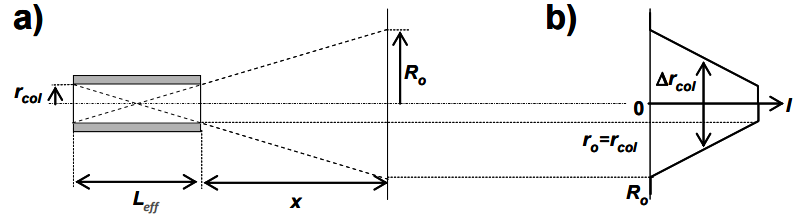
\includegraphics[width=6cm]{collimator.PNG}
\end{wrapfigure}
\grey{Parallel hole} collimator: septa parallel to each other, usually hexagonal. Thickness such that 95\% attenuation. Effective length shortened by this: \grey{$L_\mathrm{eff} = L - 2 / \mu_\mathrm{septa}$}. Resolution = FWHM\{PSF\} = \grey{$\Delta r_\mathrm{col}(x) = \frac{2r_\mathrm{col}}{L_\mathrm{eff}}(x + L_\mathrm{eff})$}.
\grey{Converging collimator}: holes focused towards body, magnifies images, increases spatial resolution.
\grey{Diverging collimator}: larger FOV, lower res., for whole body scinti.
\grey{Pinhole collimator}: very small organs, animals. significant magnification, good res., geometric distortion at image edge. Low SNR. PSF depends on source location and pinhole cone $\measuredangle$.

\subsubsection{Scintillator} NaI:Tl = Thallium activated NaI. $\gamma$-ray strikes crystal, loses energy (p.e. and compton) $\Rightarrow$ excited electronic states in crystal. \grey{Deexcitation after 230ns} $\rightarrow$ \grey{blue light @ 415nm}, 1 blue $\gamma$ / 30eV absorbed. NaI:Tl: high $\mu=2.22\mathrm{cm^{-1}}$ @ 140keV (-$>$high Z), high efficiency, transparent to 415nm, grows easily/cheaply, 415nm ideal for PMT, disadv.: hygroscopic. Tradeoff resolution / SNR: Thin crystal = narrow PSF, good res. Thick crystal = many $\gamma$ detected, high SNR. Usually \grey{thickness $\approx$ 1cm}. Efficiency \grey{$\varepsilon = 1-e^{-\mu_\mathrm{crystal}d_\mathrm{crystal}}$}

\begin{wrapfigure}[9]{l}{4cm}
	\vspace{-4mm}
	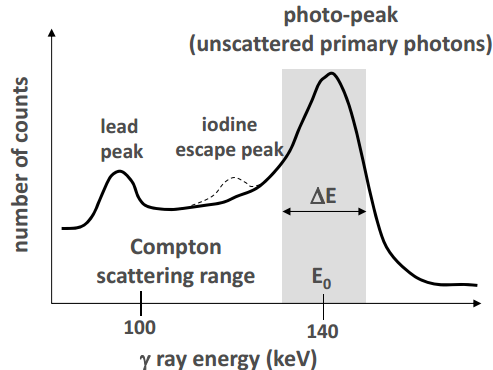
\includegraphics[width=4cm]{nuclearImagingCurve.PNG}
\end{wrapfigure}
\subsubsection{PMT}: Amplitude of signal $\propto E_\gamma$. To avoid detection of scattered $\gamma$, events binned in MCA and only a range around photopeak are counted. Usually, FWMH of photopeak $\approx$ 14keV $\hat{=} 10\%$, typically 20\% is used. $10^5-10^6$ electrons for each incident photoelectron. \grey{$\frac{\Delta E}{E_0} = 1/\sqrt{p \cdot \bar{N}_\mathrm{ph}}$}, where $p$=prob. that photoelectron is produced at PMT, $\bar{N}_\mathrm{ph}$=\# of photons per $\gamma$-photon, $\Delta E$=FWHM\{photopeak\}

\subsection{Image Quality}
\subsubsection{SNR} = $\sqrt{\mu}$ (possion statistics). Tissues deep in body: more attenuation $\Rightarrow$ low SNR. Higher dose $\Rightarrow$ more signal $\Rightarrow$ higher SNR. Collimator properties (eg. longer septa, higher res. but lower SNR). Post acquisition filtering (low pass $\Rightarrow$ higher SNR).

\subsection{Resolution}
\grey{$R_\mathrm{system} = \sqrt{R_\mathrm{gamma}^2 + R_\mathrm{coll}^2}$} $\approx$ 1-2cm(deep), 5-8mm(close). $R_\mathrm{col}$ from colimator, $R_\mathrm{gamma}$ from uncertainties in camera (accurate pos. of scintillation, error in PMT localization)

\subsection{SPECT} 
Single Photon Emission Computed Tomography. Reconstruction either like CT or iterative process: start with estimate, calculate sinogram, compare with measured sinogram; error acceptable? no: calculate update function, update estimate, start again.

\subsection{PET}
Positron Emission Tomography. Radionuclide undergoes $\beta^+$ decay (p${}^+ \rightarrow$ n + e${}^+$ + $\nu$), positron travels a bit until almost resting, then e${}^-$ + e${}^+$ $\rightarrow$ $2\gamma$ @ 511keV each.

\subsubsection{Radionucliedes} \grey{Isotope} : $\tau_{1/2}$[min] : $E_{e^+,max}$[MeV] : usage, \grey{${}^{18}$F} : 110 : 0.63 : onko/inflamm./cardiac viab., \grey{${}^{11}$C} : 20.4 : 0.96 : cardiac metab., \grey{${}^{15}$O} : 2 : 1.73 : cerebral blood flow, \grey{${}^{13}$N} : 10 : 1.2 : cardiac bl.fl., \grey{${}^{82}$Rb} : 1.3 : 2.6/3.4 : cardiac perfusion. All except Rb produced in cyclotron, Rb produced from moly-cow like generator. High $E$ $\Rightarrow$ high e${}^+$ range (ultimate resolution limit).

\subsubsection{Line Of Response}
\grey{$r=x\cos\varphi + y\sin\varphi$}. There's ${N \choose 2}$ LORs
\subsubsection{Coincidence Detection} Detection in i $\Rightarrow$ signal i set to 1 for $t$. If during $t$, detection in j, then sum of two signals goes above threshold and coincidence is counted.

\subsubsection{Detector}
Segmented block of scinti.mat. (e.g. LSO/BGO ($\mu$=0.96/mm)) with reflective mat. in cuts (deeper at edges, shallow in middle). PMTs/APDs below. Position of hit calculated from 4 signals.

\subsubsection{FWHM} discrete detector pairs: \grey{FWHM$=w\frac{r+x}{2r}$} depth dep. $\downarrow$

\subsubsection{Efficiency} 
\grey{Detection eff.} \grey{$\varepsilon = (1-e^{-\mu d})\Phi$} with $\mu,d$ scinti atten./thickness, $\Phi$ fraction of events in selected $E$ window.
Geometric efficiency: 
\begin{wrapfigure}[6]{l}{3.7cm}
	\vspace{-4mm}
	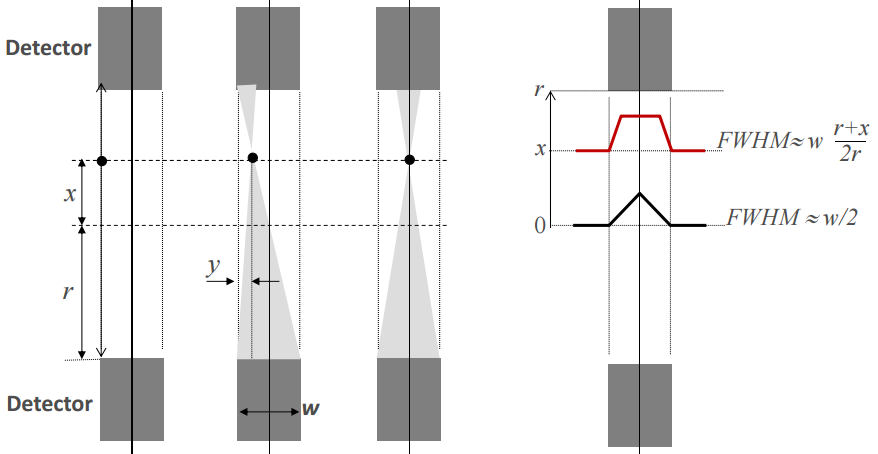
\includegraphics[width=4cm,]{petfwhm.PNG}
\end{wrapfigure}

\grey{Axial geom. coverage} \grey{$\Omega =4\pi\sin(atan({z \over d}))$}

\grey{Radial geom. coverage} \grey{$\varphi = \frac{xy}{(x+x_d)(y+y_d)}$}

\grey{Total} \grey{$\eta[\%] = 100\% \cdot \varepsilon^2 \varphi \frac{\Omega}{4\pi}$}.
$\varepsilon^2$ b/c coincidence.

\subsubsection{Normalization Correction} due to non-uniform detector efficiencies -$>$ structures in the images -$>$ compensate for the inverse of those strucures to get a corrected image -$>$ take the difference
\begin{wrapfigure}[3]{l}{2cm}
	\vspace{-6mm}
	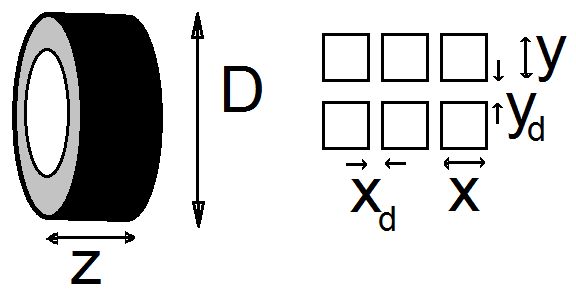
\includegraphics[width=2cm,]{geometricefficiency.png}
\end{wrapfigure}

\subsubsection{Attenuation Correction}
Correction for losses: (uniform $\mu$ assumed and traveled distance estimated). Prob. for absorption of right $\gamma$: $p_{1ij} = e^{-\mu x_{ij}}$, left: $p_{2ij} = e^{-\mu(D_{ij}-x_{ij})}$, coincidence: \grey{$p_{ij} = p_{1ij}p_{2ij} = e^{-\mu D_{ij}}$} $\Rightarrow$ attenuation correction: \grey{$a_{ij}=p_{ij}^{-1}=e^{\mu D_{ij}}$}. In PET/CT based on CT data.
\begin{wrapfigure}[3]{l}{2cm}
	\vspace{-4mm}
	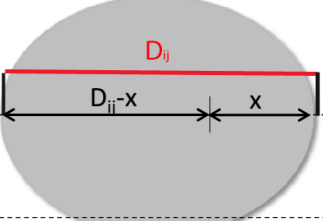
\includegraphics[width=2cm,]{attenuationcorrection.png}
\end{wrapfigure}
\subsubsection{Scatter Correction} \grey{Analytical method}: Assume scatter distribution varies slowly across medium, use phantom data to correct. \grey{Dual energy window}: Change of energy by \grey{$E_{\gamma}' = \frac{m_e \cdot c^2}{m_e c^2 / E_\gamma + 1 - \cos \theta}$}. Look at second window below p.e. peak. lower window contains scatter only, p.e. peak window true events and scatter. Projection scale$\&$subtract. \grey{Simulation method}: reconstruction w/o correction, estimation of correction in second step.

\subsubsection{Random Coincidence Correction} Frequency of randoms: $N_R = 2\tau N_1N_2$, with $2\tau$=coincidence window, $N_{1,2}$ individual detection rates. No geometrical info, almost uniform across FOV $\Rightarrow$ loss in CNR. Measure $N_{1,2}$ coincidences by disabling the synchronization of the receivers. This gives the background noise which can be subtracted afterwards. Alt. parallel coincidence circuit only rand coinc. subtract.

\subsubsection{Detector Dead Time} Components: paralysable (dead time restarts, crystal 230ns to release $e^{-}$) and non-(missed count, PHA). Loss of event counts. \grey{$N_\mathrm{measured} = N_\mathrm{true} \, e^{-N_\mathrm{true} \delta_\mathrm{dead}}$}. Particularly severe for high activities $\rightarrow$ high countrate.

\subsubsection{PHA, MCA} PulseHeightAnalyzer: receives sum contributes from MPTs and rejects scattered $\gamma$; MultipleChannelAnalyzer: A/D conv. digitizes signal and produces pulse-height spectrum ($\#$events/E)

\subsubsection{Time of Flight} Time res. $\Delta t \approx$ 500ps = 7.5cm. Improves spatial confinement, sensitivity. Requires extremeley fast scintillators.

\subsubsection{3D PET} \grey{3D slice rebinning}: Data reduced by rebinning events with azimuth of LOR $\theta\neq0$ into bins of the average $\bar{z}$. Side effect: axial misregistration. \grey{3DRP} reconstruction of N$\times$2D sinograms at azimuth $\theta=0$, estimation of missing data for $\theta>0$, forward projection. $\Rightarrow$ better statistics and thus SNR.

\subsubsection{Filtering} As high spatial frequencies are sparsely sampled, white noise stronger than signal there. Have to use filters to get rid of noise. Shepp-Logan(M)/Ramp enhance fine-structure, but also noise. Hann (lower M) decreases noise, but also resolution.
\subsection{Quantitative PET}

\subsubsection{${}^{11}$C}
\grey{${}^{14}_{\ 7}$N + p $\rightharpoonup {}^{15}_{\ 8}$O $\overset{\ll 1s}{\rightharpoondown} (\alpha \: +) \ {}^{11}_{\ 6}$C $\overset{20\mathrm{min}}{\rightharpoondown} {}^{11}_{\ 5}$B + e${}^+ + \nu_\mathrm{e}$}
Proton from cyclotron. \grey{Advantages}: In principle, all organic compounds can be labelled. Receptor affinity and Pharmacokinetic properties same as cold version $\Rightarrow$ ideal for drug testing.  \grey{Disadvantages}: chemical synthesis difficult (time, need hot cells and synthesis modules). Exposure maybe to short for enrichment at receptor $\Rightarrow$ low target to background.

\subsubsection{${}^{18}$F}$t_{1/2}$ = 110min. \grey{Advantages}: Half life long enough for synthesis and shipping. Still relatively short study repetition time possible. \grey{Disadvantage}: Pharmacokinetics different from parent compound unless already fluorinated.

\subsubsection{Injected Dose} 
\grey{$\%ID/$g$ = \frac{c_tv_t}{D_\mathrm{inj}} \frac{1}{m_t} \cdot 100\%$} with $c_t,v_t,m_t$ tissue concentration, volume, mass and $D_\mathrm{inj}$ injected dose.

\subsubsection{Stand. Uptake Value} 
\grey{SUV = [$\%ID/$g]$ / 100\% \cdot M,S$} with either $M$ total body mass or $S$ total body surface. ($<1\%$ typ.)

\subsubsection{Receptor Binding} \grey{L + R $\leftrightharpoons$ RL}. Equilibrium const. $K_d = {k_\mathrm{on} \over k_\mathrm{off}} = \frac{[L][R]}{[RL]}$. Principle of microreversability $k_\mathrm{off} [RL] = k_\mathrm{on}[R][L]$. Mass conservation $[R_T] = [R]+[RL]$. Put this in eq. const.: \grey{$\frac{[RL]}{[L]} = -\frac{1}{K_d}[RL] + \frac{[R_T]}{K_d}$} (\textbf{Scatchard equation}). For $[RL]\ll[R_T]$: $\frac{[RL]}{[L]} = \frac{[R_T]}{K_d} = \frac{B_\mathrm{max}}{K_d}$ (with $B_{max}$ the \grey{max binding capacity})

\subsubsection{Tracer Extraction}
\grey{Extraction factor $E = 1-e^{-P\cdot S / F}$} with capillary permeability $P$, cap. surface $S$, flow $F$. (Renkin-Crone).

\subsubsection{Distribution Volume} $V_d = \frac{M}{c_{bl}}$ with total amount of tracer $M$ and measured concentration in blood $c_{bl}$. Very high: tracer lipophilic, around 70L: tracer goes to lean body mass, around 5L: tracer stays in blood.

\subsubsection{Partition coefficient} $\lambda = \frac{c_t}{c_{bl}}$ with tissue concentr. $c_t$

\subsubsection{Distribution in Tissue Compartments}
4 compartment model can be simplified to 3 comp. by assuming $k_5$ and $k_6$ to be fast in comparison to the other rate constants. 
p: plasma, f: free (in tissue), ns: non-specific bound, b: bound.\\ For instant equilibration: $c_f= f_2 \cdot (c_f + c_{ns})$ with $f_2=k_6/(k_5+k_6)$ and $\dot{c_f} = k_1c_p - (k_2+k_3)c_f + k_4c_b$, $\dot{c_b} = k_3c_f - k_4c_b$. $k_1 = F\cdot E$, $k_2 = k_1 \frac{c_p}{c_f}$ (diff.outflow), $k_3=k_\mathrm{on}[R]$, $k_4=k_\mathrm{off}$. Solution: $\alpha_{1,2}=\frac{1}{2}\{k_2+k_3+k_4\pm((k_2+k_3+k_4)^2-4k_2k_4)^{1/2}\}$, $a_i=\frac{k_3+k_4-\alpha_i}{\alpha_2-\alpha_1}$
\begin{wrapfigure}[4]{l}{3cm}
	\vspace{-3mm}
	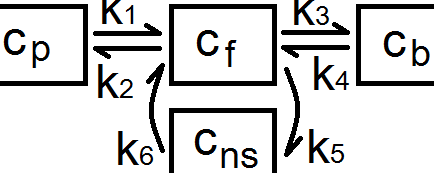
\includegraphics[width=3cm,]{tissuecompartments.png}
\end{wrapfigure}
\grey{$c_t(t)=c_f + c_b =k_1\sum_{i=1}^2 a_ie^{-\alpha_it} \ast c_p(t)$}, w/o receptor $c_t(t)=c_f(t)=k_1e^{-k_2t}\ast c_p(t)$. 

\subsubsection{Competition Between Hot and Cold Drug} $[R_T] = B_\mathrm{max}=c_b^*(t)+c_b(t)+B_\mathrm{max}'\approx c_b(t)+B_\mathrm{max}'$. Receptor occupancy for cold drug: $RO = \frac{c_b}{B_\mathrm{max}} \cdot 100\% = (1-\frac{B_\mathrm{max}'}{B_\mathrm{max}}) \cdot 100\%$. Assumptions: Same \# of receptors available for hot/cold ligands; Dose linearity $:\Leftrightarrow \frac{B_\mathrm{max}}{c_b^*} = \frac{B_\mathrm{max}'}{c_b'^*}$ Plotting $c_t(t)$, we would expect it high for compartment expressing receptor and low for not-expressing receptor (after build-up).

\subsubsection{Drug Testing} To measure behaviour of a drug (cold ligand): Make tracer (hot ligand) that goes to the same receptors. Do experiment with (-$>B'_{max}$) and without drug (-$>B_{max}$). The drug changes the \# of total receptors from $B_{max}$ to $B'_{max}$. E.g. for dopaminergic system in cerebral cortex: apply [${}^{11}$C]raclopride, binds to D${}_2$ receptors. Scan. Administer drug, displaces tracer. Scan. $\rightarrow$ determine selectivity of drug, occupancy of receptor. Similar for serotonin (5HT) with 5HT${}_2$ receptor. $\Rightarrow$ FDG6P trapped in cell. 

\begin{wrapfigure}[3]{l}{2cm}
	\vspace{-4mm}
	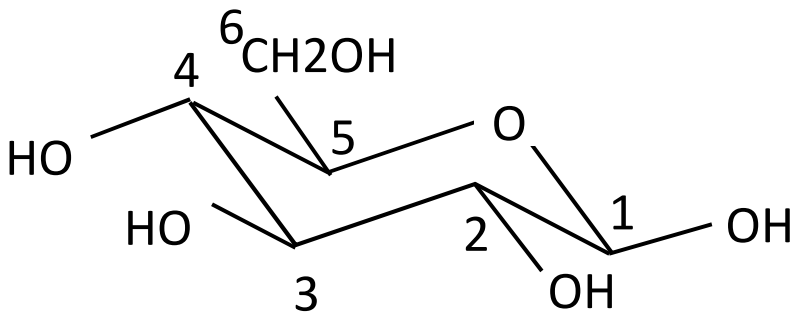
\includegraphics[width=2cm,]{glucose.PNG}
\end{wrapfigure}
\subsubsection{Glucose Metabolism} Measured with [${}^{18}$F]-2-fluoro-2-deoxyglucose (FDG). Taken up from plasma into cell ($c_p^* \overset{k_1^*}{\rightharpoondown} c_e^*$). Phosphorylated by hexokinase ($k_2^*$) like glucose (G), but not further by isomerase to fructose. 
Metabolic rates FDG/G: \grey{$\nu_\mathrm{FDG}^\mathrm{MR} = k_2^*c_e^*(t) \approx \frac{k_1^*k_2^*}{k_{-1}^*+k_2^*}c_p^*(t)$}.
\grey{$\nu_\mathrm{G}^{MR} \approx \frac{1}{LC} \nu_\mathrm{FDG}^\mathrm{MR} \frac{c_p(t)}{c_p^*(t)}$}.

\begin{wrapfigure}[8]{l}{5cm}
	\vspace{-4mm}
	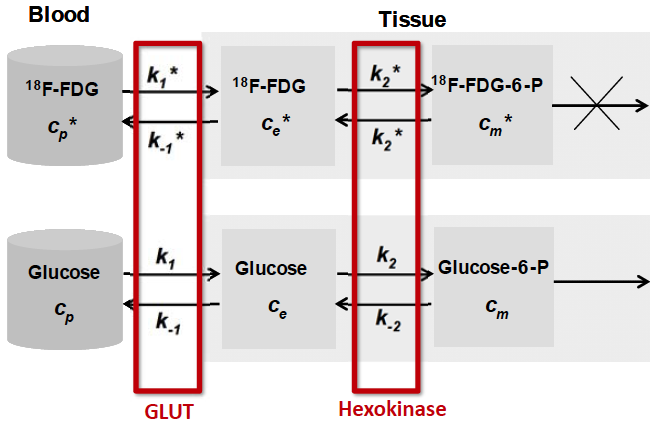
\includegraphics[width=5cm,]{FDG-Metabolism.png}
\end{wrapfigure}
\vspace{-1mm}

$LC\in[0.3,0.8]$: correction to translate measured $\nu_\mathrm{FDG}^\mathrm{MR}\rightarrow$G. \grey{Usage}: brain metabolism (e.g. reduced activity in alzheimer), detection of metastatic lesions (tumors have higher anaerobic glycolytic rates). (fig: GLUT and Hexokinase)

\vspace{3mm}
\section{MRI}
\vspace{-3mm}
Magnetic moment \grey{$\vec \mu = \gamma \vec S$} with gyromagnetic ratio $\gamma$ ($\mu _z = \pm \gamma \hbar /2 $). $\frac{\gamma}{2\pi}$ in MHz/T: ${}^1$H=42.6, ${}^{13}$C=10.71, ${}^{19}$F=40.07, ${}^{31}$P=17.24

Energy of spin in $\vec B || \hat{z}$: \grey{$E=-\vec\mu \cdot \vec S = -\mu_zB_0 = \pm \frac{\hbar}{2} \gamma B_0$}. Population of up/down states follows Boltzmann statistics: \grey{$\frac{n_\mathrm{down}}{n_\mathrm{up}} = e^{-\Delta E / k_\mathrm{B} t}$}. $\Delta E= \hbar \omega _L$ To faciliate transitions irradiate at Larmor frequency: \grey{$\omega_L = \gamma B_0$}. Net magnetic moment: \grey{$\vec M_0 = \sum \mu_i = \Delta n \mu_z$}, \grey{$\frac{\Delta n}{n}=\frac{\gamma \hbar B_0}{2 k_b T}$}

\grey{tissue} : T1 @ 1.5T : T1 @ 0.5T : T2 [ms], \grey{WM} : 790 : 539 : 92, \grey{GM} : 920 : 656 : 100, \grey{CSF} : $>$2500 : $>$2500 : $>$2000, \grey{Skeletal muscle} : 870 : 600 : 47, \grey{Liver} : 490 : 320 : 40, \grey{Fat} : 260 : 215 : 85
\subsection{Bloch Equations}
\vspace{-1mm}
\scalebox{0.7}{ \grey{$\frac{d}{dt}\vec{M} = \left( \begin{matrix}
						-1/T_2 & -\gamma B_z & \gamma B_y \\
						\gamma B_z & -1/T_2 & -\gamma B_x \\
						-\gamma B_y & \gamma B_x & -1/T_1\end{matrix} \right) \vec{M} + \left( \begin{matrix}
						0 \\ 0 \\ M_0 / T_1 \end{matrix} \right)$}} Rotation: $\vec M$ rotates around $\vec B$ with $\omega=\gamma|B|$, spin-spin relaxation (transverse components decay with $R_2=1/T_2$), spin-lattice relaxation ($z$-component returns to $M_0$ with $R_1=1/T_1$).
Transverse component effectively decays faster because of phase coherence loss (b/c inhomogenities in $B_0$). $T_2^* = (1/T_2^+ + 1/T_2)^{-1}$ \grey{$M_z(t)= M_0-M_0(1- cos(\alpha))(1-exp(-t/T_1))$} \grey{$M_y(t)=M_0sin(\alpha)exp(-t/T_2)$}

\subsubsection{Magnetisation Manipulation}
Apply external $B$-field rotating in $xy$ at Larmor frequency: $B_{x,y} = B_1 \cos,\sin(\omega_Lt)$. \grey{Tip angle $ \alpha =\gamma B_1 \tau _{B1}$}. Signal is maximized at the \grey{Ernst angle: $\alpha _E = arccos(e^{-T_R/T_1})$}. In rotating frame, $\vec M$ then rotates around $\vec B_1'$ with $\omega = \gamma B_1$. (Assuming $t_\mathrm{excitation} \ll T_{1,2}$); correction: $B_z=B_0-\omega_{RF}/\gamma$. 

\subsubsection{Detection of Precession}
Faraday: 
\grey{$\oint_{\del S} \vec E(\vec r, t) \dif \vec r$} \grey{$= - \frac{\dif}{\dif t} \iint_S \vec B(\vec r, t) \dif \vec \sigma$}.
Use with conductive loop. Rotating magnetisation in volume $V$ at $\vec r_0$ generates magnetic field $\vec B(\vec r, t) = \hat{\vec B}(\vec r) e^{i\omega t}$ which induces $\hat U_\mathrm{ind} = i\omega \int_\mathrm{coil} \hat{\vec B} (\vec r) \dif \vec A$. For transmit field $\vec B^t (\vec r_0)$ driven with $I_0$, $U_\mathrm{ind} = i\omega I_0^{-1} \hat{\vec{\mu}} \cdot \hat{\vec B^t(\vec r_0)}$.
With $\vec \mu = V (M_{xy}, -iM_{xy}, 0)^T$, 
we have $U_\mathrm{ind} = M_{xy} V i \omega B_1^{(-)}$ 
and coil sensitivity \grey{$s(\vec r) = i \omega B_1^{(-)}$} with \grey{$B_1^{(-)} = I_0^{-1}(\hat B_x^t(\vec r) - i \hat B_y^t(\vec r))$}. Circular current: \grey{$\hat{\vec B} (\vec r) = \frac{\mu \hat I}{4\pi} \oint_C \frac{\dif \vec l \times (\vec r - \vec r_l)}{|\vec r - \vec r_l|^3}$} (Biot-Savart), works well for low freq./quasi stationary approx., for sample size $\ll$ $\lambda$. (@7T:$\lambda$=13cm).$\uparrow$ $D_{coil}$  $\rightarrow$ Depth $\uparrow$ Sensitivity $\downarrow$

\subsubsection{Free Induction Decay}
After turning off $B_1$, signals in $x$ and $y$ are oscillation enveloped by exponential decay. Spectrum = Lorentz peaks from water and lipid (lower freq.) with $FWHM = 1/(\pi \cdot T_2^*)$.
\vspace{-2mm}
\subsection{Noise} 

\subsubsection{Resistor Voltage Noise} \grey{$\sigma_\mathrm{noise}^2 = 4k_B\,T\,R\,BW$} (Johnson, Nyquist). Equivalent R of sample: Current $I_0$ generates field $\vec E$, dissipated power $P = \iiint \sigma(\vec r)|E(\vec r)|^2 \dif V$ $\Rightarrow$ \grey{$R = \frac{P}{I_0^2}$}. 
J.N. assumes constant R across BW (but receiver coil is tuned circuit) and T across setup (but 310K for body, 77K+ for coil). 
Eff. R: $R_\mathrm{sample}^\mathrm{eff} = \frac{1}{2\pi\,BW} \int_\mathrm{sample}\int_{\omega_1}^{\omega_2}\frac{\sigma(\omega,\vec r)|\vec E(\omega, \vec r)|^2}{I_0^2}\dif\omega\dif V$
$\Rightarrow$ \grey{$\sigma_\mathrm{noise}^2 = 4k_B\,BW (R_\mathrm{sample}^\mathrm{eff}T_\mathrm{sample} + R_\mathrm{coil}^\mathrm{eff}T_\mathrm{coil} + R_\mathrm{env}^\mathrm{eff}T_\mathrm{env})$}.
Reducing noise: Reduce BW (but longer scan time), T (impractical) or R (copper/silver for coil, cool). Effects of magnetic field neglegible (true for biol. samples). Sources are: electric charges and dipoles.

\subsubsection{SNR}
\grey{$= \frac{U_\mathrm{signal}}{\sigma(U_\mathrm{noise})} = \frac{\omega B_1^{(-1)}(\vec r)M_{xy}(\vec r)\Delta V}{\sqrt{4k_B \mathrm{BW}(T_\mathrm{sample}R_\mathrm{sample} + T_\mathrm{coil}R_\mathrm{coil})}}\sqrt{N_\mathrm{avg}}$}
SNR $\propto \Delta V \sqrt{t_\mathrm{scan}}$. Increasing SNR: \grey{Signal side}: increase $B_1^{(-)}(\vec r)$ (e.g. smaller TX coil), increase magnetization $M_{xy}(\vec r) \propto B_0$, increase frequency $\omega \propto B_0$. \grey{Noise side}: above.

\subsubsection{Resolution}
\grey{Relaxation limit}: If data acq. long relax. $H(k) = \mathrm{rect}(\frac{k}{2k_\mathrm{max}})e^{-\frac{t}{T_2^*}}$ $\Rightarrow$ (FT = sinc$\ast$Lorentz) \grey{$\Delta x \geq \mathrm{FWHM} = \frac{\pi}{\gamma G_\mathrm{max} T_2^*}$} Sol. $t_{scan} \downarrow$ G $\uparrow$.
\grey{Diffusion limit}: $\langle \Delta x^2 \rangle = 6DT_\mathrm{ACQ}$ $\Rightarrow$ (with $D = 10^{-3}\frac{\mathrm{mm}^2}{\mathrm{s}}$ and $T_\mathrm{ACQ}$ = 10ms) \grey{$\Delta x \geq 8\mu\mathrm{m}$} eq. valid 4 free diff.

\subsection{Image Acquisition}
\begin{wrapfigure}[6]{l}{1.3cm}
	\vspace{-4mm}
	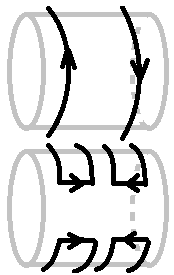
\includegraphics[width=1.3cm,]{maxwellgolay.png}
\end{wrapfigure}
Assuming axial slice with normal in $z$.
\subsubsection{Field Gradients}
Maxwell pair in $z$, Golay pairs in $x,y$. \grey{$G_i = \frac{\del B_z}{\del i}$}.

\subsubsection{Slice Selection}
Apply $G_z$, send in 90${}^\circ$-pulse with bandwidth $\Delta \omega_s$ centered at $\omega_s = \omega_L(z=\mathrm{slice\ centre})$. Ideal RF-excitation to achieve this frequency profile: $B_1(t)= K \cdot sinc(\Delta \omega _s \pi t) \cdot sin(2\pi \omega _s t)$. Slice thickness \grey{$T = \frac{2\Delta\omega_s}{\gamma G_z}$}. During $\tau_\mathrm{grad}$(small to avoid M attenuation), different phases accumulate in the slice $\varphi_\mathrm{slice}(z) = \gamma G_z z \tau_\mathrm{grad}\textit{/2}$ $\rightarrow$ rephasing gradient $G_z^\mathrm{reph} = \frac{\tau_\mathrm{grad} G_z}{2 \tau_\mathrm{reph}}$ to avoid signal loss (M). $\varphi_\mathrm{slice}(z)$ is due to \grey{Fourier Slice Theorem}: frequency shift $\rightarrow$ phase increases linearly.

\subsubsection{Phase Encoding}
During time $\tau_\mathrm{pe}$, $G_y$ is switched on. Spins precess with $\omega(y) = \gamma G_y y + \omega_0$ and acquire different phases $\varphi_\mathrm{pe}(G_y, \tau_\mathrm{pe}) = \gamma G_y y \tau_\mathrm{pe}$.

\subsubsection{Frequency Encoding}
During signal acquisition, $G_x$ is turned on. Spins precess with $\omega(x) = \gamma G_x x + \omega_0$ and thus the spectrum represents a projection of $xy$ onto $x$. For image with \grey{$N_x\times N_y$} pixels, signal is sampled $N_x$ times and whole process is repeated $N_\mathrm{pe}=N_y$ times with different $G_y$, taking a total time $T=T_\mathrm{rep} N_\mathrm{pe}$ where the repetition time $T_\mathrm{pe}$ needs to be long enough to allow for sufficient $T_1$ relaxation.

\subsubsection{k-Space Formalism}
.\\
Signal: $s(G_y,\tau_\mathrm{pe},G_x,t) \propto \iint \rho(x,y) e^{-i\gamma G_y y \tau_\mathrm{pe}} e^{-i\gamma G_x x t} \dif x \dif y$ \\
Spatial frequencies: \grey{$k_x = \frac{\gamma}{2\pi}G_xt, \ k_y=\frac{\gamma}{2\pi}G_y\tau_\mathrm{pe}$} \\
$\Rightarrow$ \grey{$S(k_x, k_y) \propto \iint \rho(x,y)e^{-i2\pi k_xx}e^{-i2\pi k_yy} \dif x\dif y = \fcal\{\rho(x,y)\}$}

\subsubsection{Object- vs k-Space}
Voxel size \grey{$\Delta x = \frac{\mathrm{FOV}_x}{N_x}$}. Sampling distance k-space: \grey{$\Delta k_x = \frac{\mathrm{BW}_x}{N_x} = \frac{2\pi}{\mathrm{FOV}_x}$}. Resolution in one space translates to extent in other and vice-versa.

\subsubsection{Traversing k-Space speed} 
\grey{$\dot{\vec k} = \gamma \vec G(t)$} $\vec{G}$ gives direction

\subsubsection{Imaging Sequences}
\vspace{-4.5mm}
\begin{figure}[H]
	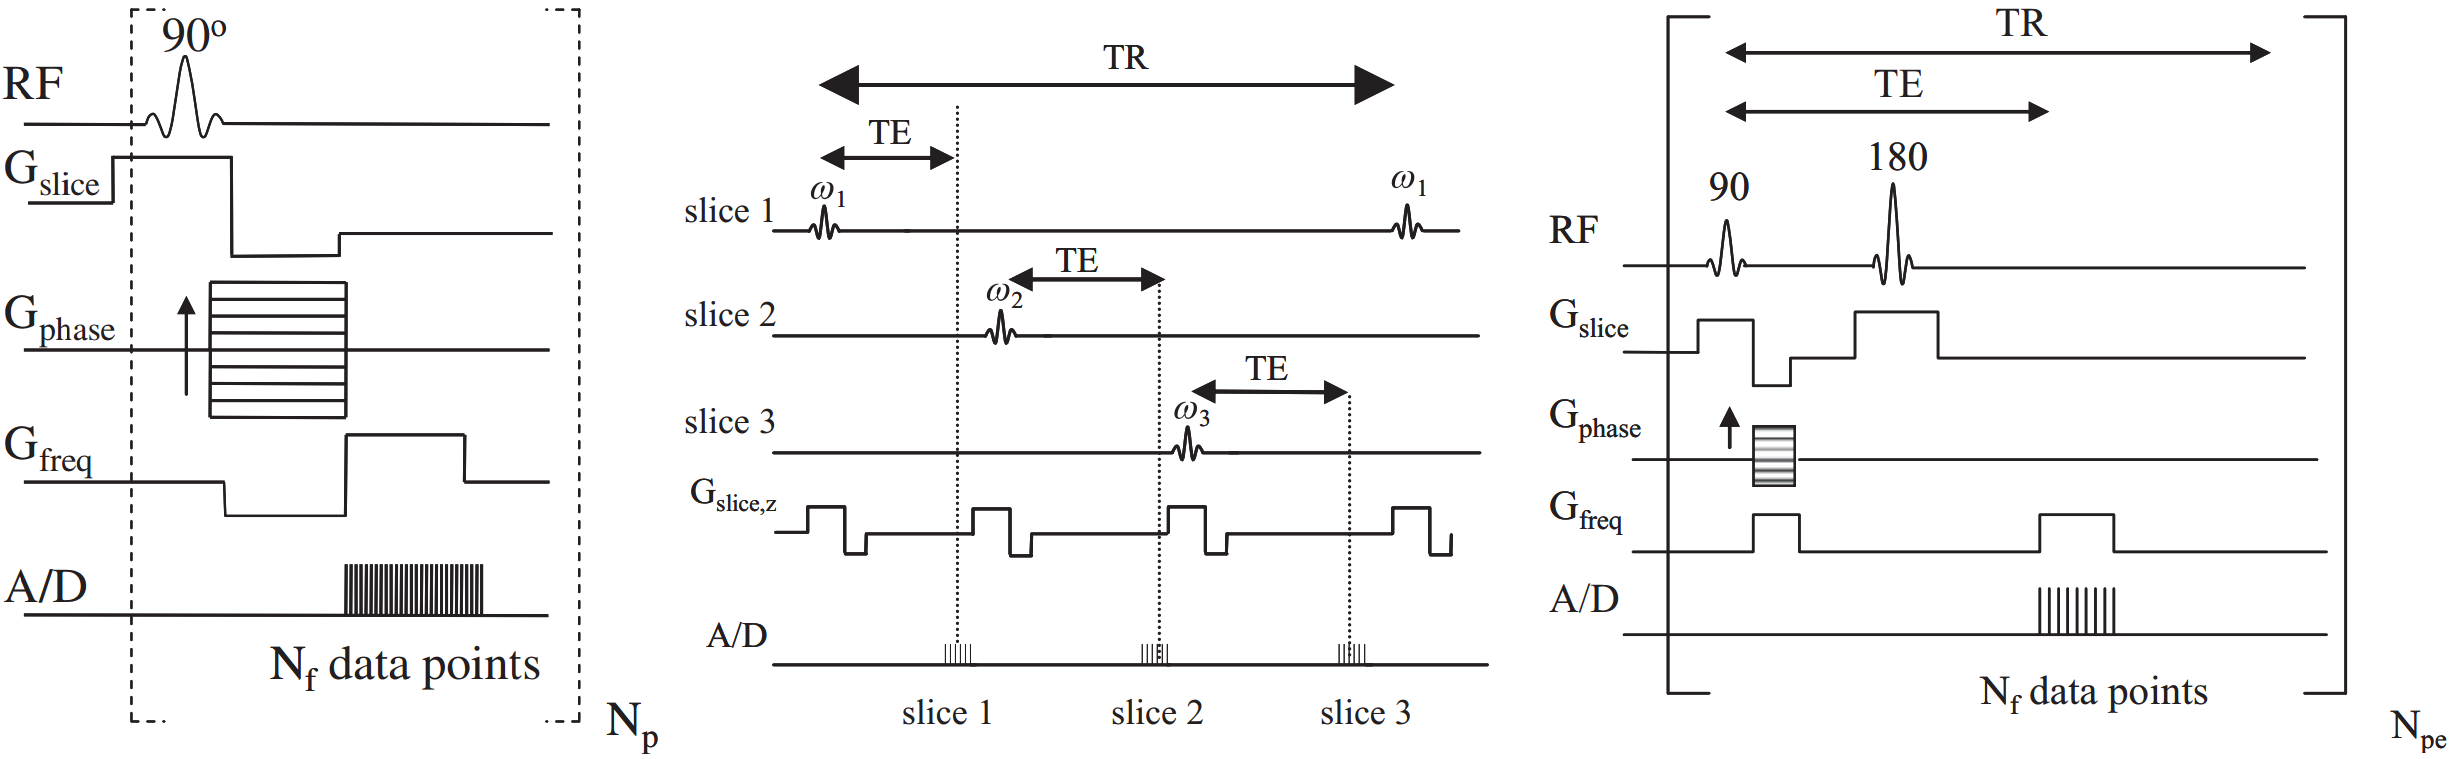
\includegraphics[width=0.4\textwidth]{sequences.png}
\end{figure}
\vspace{-5mm}
\grey{Gradient Echo Imaging}: Most basic and fastest. Scan one line of k-space, wait until repetition time over (as $T_2^* \ll T_1$, TE$<$TR), scan next line. Image intensity 
\grey{$I(x,y) \propto \rho(x,y)\frac{(1-e^{-\frac{\mathrm{TR}}{T_1}})\sin\alpha}{1-e^{-\frac{\mathrm{TR}}{T_1}}\cos\alpha}e^{-\frac{\mathrm{TE}}{T_2^*}}$ }
with the magnetisation angle $\alpha$. Maximal intensity for given TR for ernst angle.
\grey{Multi-slice G.E. imaging}: waiting time: TR-TE $\rightarrow$ max $\#$ slices: TR/TE. Scan line 1 of slice 1, then immediately l1s2, l1s3, ..., after TR is up l2s1, l2s2, ... or interlaced fashion (even,odd)
\grey{Spin echo} Disadvantage G.E.: cannot weight by $T_2$, only $T_2^*$ $\rightarrow$ reverse phase coherence loss with 180${}^\circ$ pulse after slice selection, phase encoding and prephasing, then waiting for same time before ACQ. \grey{$\vec k \rightarrow -\vec k$ in the k-space}, thus prephasing (goint to left of BW) must happen with same gradient sign as during ACQ. Intensity: \grey{$I(x,y) \propto \rho (x,y)(1-e^{-\frac{\mathrm{TR}}{T_1}})e^{-\frac{\mathrm{TE}}{T_2}}$}. \grey{Echo Planar Imaging}: Scan multiple lines per excitation (after ACQ, go to next line with $G_\mathrm{pe}$).\grey{Turbo Spin Echo}: Same as EPI, but with additional $180^\circ$-pulses before each ACQ (T2 weighting $\uparrow$ /suscept. $\downarrow$) \grey{Inversion Recovery}: a SE seq. preceded by $180^\circ$ RF pulse. Elapsed \\
\\
time between the $180^\circ$ and $90^\circ$, TI (inversion). We can suppress fat (Short tau IR STIR) or fluid (Fluid attenuation IR, FLAIR, or double IR, DIR). Sh. TI, longer T1 contribute to T2 contrast. Magnitude reconstruction ($|M_z|$ null dark)  or phased-sensitive IR (neg $M_z$ dark).
\subsubsection{Weighting} 
\grey{Proton Density}: TE $\ll T_2^* \ \& \ (\alpha \ll \alpha_\mathrm{Ernst} | $TR $\gg T_1)$. \grey{$T_1$}: TE $\ll T_2^* \ \& \ (\alpha \sim \alpha_\mathrm{Ernst} \ | \ $ TR $ \sim T_1)$. \grey{$T_2^*$}: TE $> T_2^* \ \& \ (\alpha \ll$ 
$\alpha_\mathrm{Ernst} | $TR $\gg T_1)$. 
\grey{mixed $T_1$ and $T_2^*$}: TE $> T_2^* \&	(\alpha \sim \alpha_\mathrm{Ernst}|$TR $ \sim T_1)$.

\subsubsection{MR Angiography} 
$T_1^\mathrm{eff}$ of blood smaller, because during TR, new unsaturated blood flows into slice. $T_1^\mathrm{eff} = (\frac{1}{T_1} + \frac{v_\mathrm{blood}}{d_\mathrm{slice}})^{-1}$. Use heavily $T_1$-weighted seq (sh. TR and lar. $\alpha$). $v_b \cdot TR > S_{th}$ $\rightarrow T_1=0$

\subsubsection{Contrast Agents}
Based on Gadolinium ion in chelate. One electron binding site not occupied, which water can
temporarily bind to and undergo rapid $T_1$ relaxation.

\subsubsection{fMRI}
Blood oxygenation level dependent (BOLD) effect. Neural activity $\rightarrow$ increased blood flow and thus oxygenation. DeoxyHb is paramagnetic (oxyHb diam.), disturbs local m field $\Rightarrow$ shorter $T_2^*$ and broad dist. res. f. Use EPI (short TE) for speed. Changes in intensity only $\approx$ 0.3-5\%, $\rightarrow$ repeat stimulation/baseline several times. Detect active regions in response to stimulus $\rightarrow$ corr. $\%$ Bold response

\subsubsection{Diffusion Weighted Imaging}
Employ $90^\circ$, switch on gradient, different phases accumulate. $180^\circ$, wait same time. All phases back to 0, except for protons that diffused away from initial location, which decreases signal.
\grey{Diffusion Tensor Imaging}: Ellispe to show diffusion direction. Signal depending on diffusion tensor $T$ and gradient $\vec G$: $S(\vec G) \propto e^{-b \vec G^T \underline{D} \vec G}$. b-value: how strong and how long G on (s/$mm^2$) if $\uparrow$ b, sig $\downarrow$. depending on measurement parameters. Measure for different $\vec G$, solve for $D$. Anisotropic diff. we have a preferential direction $\rightarrow$ connectivity map (axons wrapped myelin, hydrophobic). for restricted diff. $R= \sqrt{2 \cdot D \cdot \Delta}$, $D = \lambda \cdot v/6$, $\lambda$ free path length, v mol. velocity. 

\subsection{Instrumentation}
\subsubsection{Magnets}
Outermost layer: $B_0$ magnet, cryogenics. Further in: Gradients (Maxwell and Golay pairs, see above). Innermost: RF body coils (birdcage built into MRI, almost always used for TX, smaller localized coils for RX).

\subsubsection{Stray Fields}
strongly shielded by shield coils. 5Gauss=0.5mT (kills pacemakers, magnetstrips) $\sim$ 5m from MRI. 50Gauss (mag.obj. become projectiles) 2m from MRI.

\subsubsection{Peripheral Nerve Stim.} gradient fields may cause E field loops (Eddy currents) which give a $\Delta V$ across the membrane $\rightarrow$ causes AP. The factor of cardiac nerve stim. is 80-times higher than per. nerves. Safety limit: \grey{$\sqrt{\sum (w \frac{\del B}{\del t})^2} < 20 \mathrm{\frac{T}{s}}(1 + \frac{0.36\mathrm{ms}}{t_s})$}
\vspace{-2mm}
\section{Ultrasound}
\vspace{-2mm}
Speed: \grey{$c = 1/\sqrt{\kappa\rho}$} P: \grey{$p = \rho c u_z$}
Impedance: \grey{$Z = p/u_z = \rho c = \sqrt{\rho/\kappa}$} Intensity: \grey{$I = p u_z/2$} WL: \grey{$\lambda = {c/\nu} = {1/(\nu \sqrt{\kappa \rho})}$} Part.vel: \grey{$u_z=\sqrt{2I/Z}$}

\subsection{Some Material Properties}
Subst(Z[kg/m${}^2$s] ; $\rho$ [g/cm${}^3$]; c [m/s]); Water(1.48 $\cdot 10^6$; 1.0;	1480); Muscle(1.66 $\cdot 10^6$; 1.06	; 1568); Bone(6	 $\cdot 10^6$; 1.3	-1.8; 2800-4100); Air(400(!); 0.0012; 330); PZT-5 Ceramic(29	$\cdot 10^6$; 7.65; 3790)
%\begin{tabular}{l l l l}
%Subst.			& Z	[kg/m${}^2$s] 		&$\rho$ [g/cm${}^3$]	& c [m/s]      	 	\\
%\hline
%Water			&	1.48 $\cdot 10^6$	&	1.0			&	1480        \\
%Blood			&	1.65 $\cdot 10^6$	&	1.06		&	1560        \\
%Brain			&	1.58 $\cdot 10^6$	&	1.03		&	1530        \\
%Fat			&	1.36 $\cdot 10^6$	&	0.92		&	1476        \\
%Muscle			&	1.66 $\cdot 10^6$	&	1.06		&	1568        \\
%Bone			&	6	 $\cdot 10^6$	&	1.3	-1.8	&	2800-4100   \\
%Air				&	400	(!)				&	0.0012		&	330         \\
%Epoxy			&	3	$\cdot 10^6$	&	1.2			&	2500        \\
%Plexiglass		&	3.2	$\cdot 10^6$	&	1.18		&	2730        \\
%PZT-5 Ceramic	&	29	$\cdot 10^6$	&	7.65		&	3790        \\
%Steel			&	39	$\cdot 10^6$	&	7.7			&	5000        
%\end{tabular}

%\subsection{Acoustic Windows}
%%\vspace{-5mm}
%\begin{figure}[H]
%	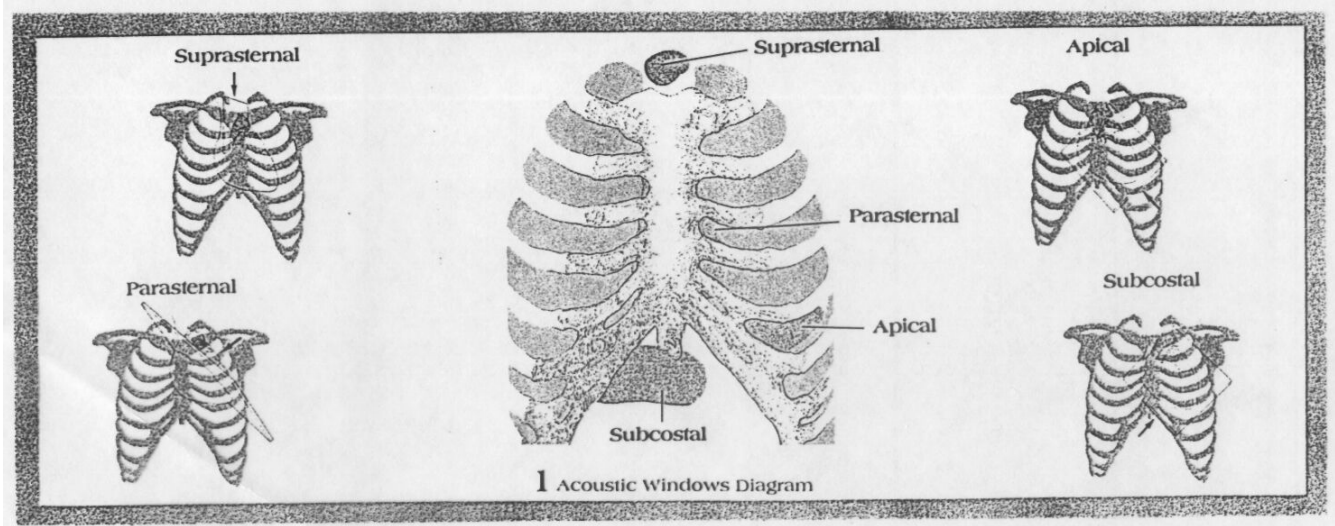
\includegraphics[width=9cm]{acousticwindows.png}
%\end{figure}
%%\vspace{-3mm}

\subsection{Fresnel Equations}
\begin{tabbing}
$R_p = {p_r \over p_i} = \frac{Z_2 \cos\theta_i - Z_1 \cos\theta_t}{Z_2\cos\theta_i + Z_1\cos\theta_t}$
\hspace{5mm} \= $T_p = {p_t \over p_i} = \frac{2 Z_2 \cos\theta_i}{Z_2\cos\theta_i + Z_1\cos\theta_t}$ \\
$R_I = {I_r \over I_i} = \frac{(Z_2 \cos\theta_i - Z_1 \cos\theta_t)^2}{(Z_2\cos\theta_i + Z_1\cos\theta_t)^2}$
\> $T_I = {I_t \over I_i} = \frac{4Z_1Z_2\cos^2\theta_i}{(Z_2\cos\theta_i + Z_1\cos\theta_t)^2}$ \\
$T_p = R_p + 1$
\> $T_I = 1-|R_I|^2$ \\
\end{tabbing}
\vspace{-4mm}
\subsection{Scattering}
\grey{Rayleigh scattering}, if $d \ll \lambda$. Then $E_\mathrm{scatter} \propto \lambda ^{-4}$ and slightly more backscatter than forward.
If objects close together, backscatter adds up constructively ($\rightarrow$Doppler US), if further apart, con/destructive interference leads to \grey{speckle} (char. wavelength: $\lambda /2$), image has granular appearance; reduced w \grey{compound img}. \grey{clutter} signal arises from side/grating lobes reflection, reduced with \grey{harmonic img}. These 2 reduce SNR/CNR.

\subsection{Attenuation}
\grey{$I(z)=I_0e^{-\mu z}$} with \grey{$\mu \: [\mathrm{dB\,cm^{-1}}] = 4.343 \mu \: [\mathrm{cm^{-1}}]$}; $p(z) = p_0 e^{-\alpha z}$\\
$\mu = 2\alpha$;
%\begin{tabular}{||}
%material			& attenuation [dB/(cm MHz)] \\
%\hline
%kidney, brain ca. 	& 1.0         \\
%liver 				& 0.8 - 1.3   \\
%skeletal muscle 	& 1.5 - 2.2   \\
%fat ca. 			& 0.5         \\
%bone ca. 			& 13          \\
%\end{tabular}
Material [attenuation in dB/(cm MHz)]: kidney\&brain [1.0], \\ liver [0.8-1.3], muscle [1.5-2.2], fat [0.5], bone [13]

\subsection{Transducer}
Piezo from lead zirconate titanate (PZT). Matching layer with \grey{$Z = \sqrt{Z_{PZT} Z_{skin}}$}, $d= \lambda _{US} /4$. Damping behind PZT to decrease ringing and allow short pulses (\grey{axial res. $\propto$ pulse length}), also increases resonator bandwidth.

\subsubsection{Beam Geometry}
Near-field = Fresnel zone: complicated wave pattern with lots of zeros in intensity, unsuited for diagnostics. Far-field = Fraunhofer zone: intensity decays exponentially. Boundary at \grey{$Z_\mathrm{NFB} \approx r^2 / \lambda$} with the transducer radius $r$. At NFB: beamwidth approx. equal to $2r$, afterwards divergence with \grey{$\theta = \arcsin(0.61\lambda / r)$}. In far-field, lateral beam shape is Gaussian. \grey{Lateral resolution = FWHM = 2.36$\sigma$.} \grey{Axial resolution $\Delta z = t_{pulse}\,c / 2 = L_{pulse} / 2$}. Implies $\Delta z \ge \lambda/2$. Typically 1.5mm@1MHz, 0.3mm@5MHz.

\subsubsection{Focusing}
Focusing by lenses or concave transducer face.
Strong focusing $\Rightarrow$ good lateral resolution at focal point, big divergence. Weak focusing $\Rightarrow$ medium lateral resolution, longer focal depth. \grey{f\# = focal distance / diameter of transducer}. Lateral resolution \grey{$\lambda f\#$}.
\subsubsection{Linear Arrays}
128-256 transducers in flat array. Typical dim: 10-15cm $\times$ 1cm. Pitch (period) $\approx \lambda$. Kerf (spacing of transducers) $\approx 30\mu$m.
Operated one to few transducers at a time. Sweep left $\rightarrow$ right. Lateral resolution limited by pitch, but small pitch $\Rightarrow$ small $\theta$.

\subsubsection{Phased Array}
Smaller and more densly packed transducer. Pitch $< \lambda / 2$. Beam focusing and steering happens by phasing the output of different transducer elements.
Small aperture and beam steering $\Rightarrow$ looking through acoustic windows possible.

\subsubsection{Receiver Beam-Forming}
TX and RX with same beam direction and focus. Analog: phased RX signal combination with delay lines, 1 signal recorded. Digital: all channels recorded, combination later.

\subsubsection{Beam steering}
Steer the beam by $\phi$ by applying a phase diff of $\Delta \phi = -kysin(\alpha)$ to each transducer, y its y-coordinate.

\subsubsection{Beam focusing}
Focusing is achieved by phasing the array elements such that their partial waves have equal phase at the focus point: $\Delta \phi = -k\sqrt{y^2+(d/cos(\alpha))	^2+2yd\sin(\alpha)/cos(\alpha)} \approx -k \sqrt{y^2 + d^2}$ with d the focus distance along the x dir.
\subsubsection{Multidimensional Arrays}
Few rows in elevation direction allows some focusing (1.5D array). Large number of rows allows steering and focusing in both directions (2D array).

\subsubsection{Grating Lobes}
Channel-to-channel phase increment: \grey{$\Delta\phi \mod 2\pi= k d \sin\alpha$} with $\alpha = \measuredangle$(transducer normal, wave propagation) and pitch $d$. $\Rightarrow$ To avoid side lobes ensure \grey{$d \leq \lambda / 2$}

\subsection{Time Gain Compensation}
Signals arriving later are amplified more strongly, counteracting the exponential attenuation in tissue and reducing dynamic range.

\subsection{SNR}
\grey{S/N = dyn. range - attenuation - loss from reflection} [dB]
dynamic range [dB] = $10 \log(P_\mathrm{tx} / P_\mathrm{noise})$
reflection loss [dB] = 20 log(loss [\%])

\subsection{Scanning Modes}
\subsubsection{A-Mode} 
Scans only one line. Mainly in opthalmology.

\subsubsection{M-Mode}
Records motion by recording A-spectra and plotting them (brightnesscoded) against time.

\subsubsection{B-Mode} 2D image by scanning each line as A-mode. Steering electronic for line/phased arrays, mechanical for annular.

\subsubsection{Scanning Procedures}
Parallel scan for large acoustic windows, sector scan (lines fanning from transducer) for small acoustic window, radial scan for inside of vessels. \grey{Compound scan} acquired from multiple angles by phased array and different beam forming schemes to average out speckle, make boundaries $\parallel$ beam visible and reduce acoustic enhancement/shadowing (after low/high attenuating tissue).

\subsection{Doppler Ultrasound}
Erythrocytes $\approx 7\mu$m, US $\lambda \approx$ 0.1-1mm
Observer receives: $f^{eff}=f_i\frac{c+v}{c}$\\
$f_{rec} = \frac{f_i (c + v\cos\theta)^2}{c^2} \Rightarrow \Delta f = f_{rec} - f_i \approx \frac{2 f_i v \cos\theta}{c}$ 
$\Rightarrow$ \grey{$v = \frac{c \: \Delta f}{2 f_i \cos\theta}$} with flow velocity $v$, recorded/initial frequencies $f_{rec,i}$, Winkel $\theta = \measuredangle(\vec v,$ beam)
(recorded with Bmode prev)
Frequency shifts on order of 0.05\%, use high frequency so the backscatter is stronger ($\propto \omega^2$), make sure $\theta$ small. \textbf{CW Doppler:}
%\subsubsection{CW Doppler}
Used when there's no need to localize source. Half of transducer elements used for transmission, half for reception. Not limited to maximal depth or flow velocity. Received signal is demodulated with transmission, which shifts spectrum such that $f_i \rightarrow 0$ and $f_i + \Delta f \rightarrow \Delta f$, but also introduces harmonics ($2f_i$ and $2f_i + \Delta f$), filtered out by LPF. Scatter from stationary structures filtered out by HPF.  \textbf{Quadrature Demodulation:}
%\subsubsection{Quadrature Demodulation}
If demodulation happens with $\cos$ only, one gets $|\Delta f|$. To differentiate between positive and negative doppler shift one takes two time-domain multiplication: one with the original transmitter waveform and one with the same waveform shifted by 90º in phase. With the cos and sine one is able to create an exponential $\rightarrow$ a single Dirac peak with a meaningful negative range of the spectrum. \textbf{Flow Profiles:}
%\subsubsection{Flow Profiles}
Laminar flow: at lower velocities, flat Doppler spectrum distribution up to $f_{max} \hat{=} v_{max}$. Plug flow: at higher speeds (eg. systole), distinct peak in spectrum. \textbf{Time-resolved Frequency Analysis:}
%\subsubsection{Time-resolved Frequency Analysis}
Weight continuous signal with $\cos^2$-window, perform FFT. \textbf{Sonogram:}
%\subsubsection{Sonogram} 
Color code amplitude, plot freq against time.
%\begin{wrapfigure}[11]{l}{7cm}
%	\vspace{-5mm}
%	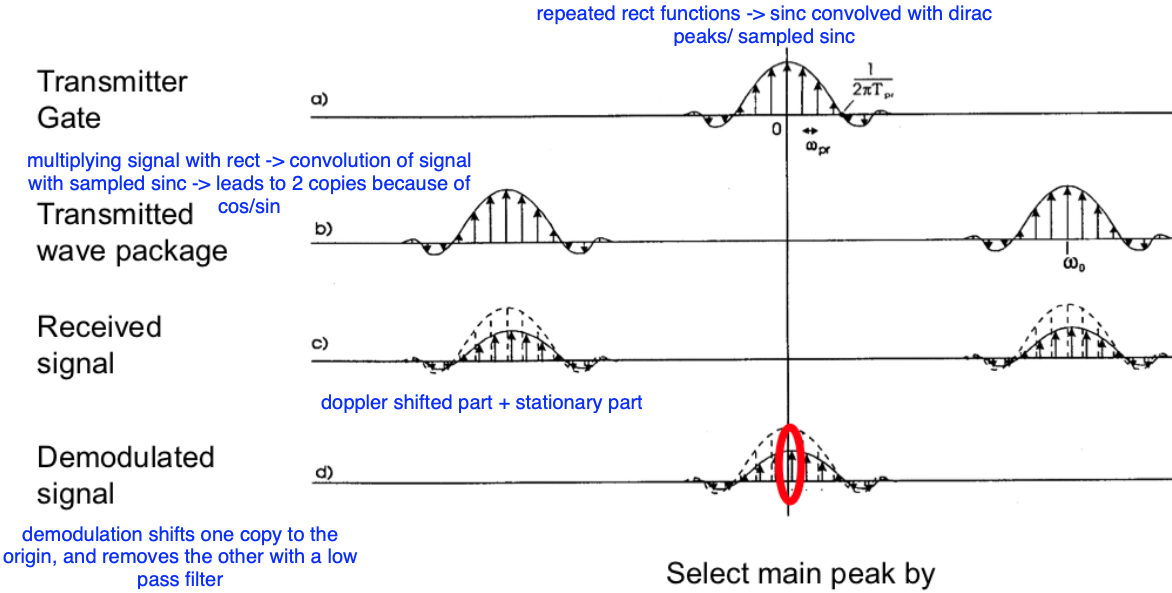
\includegraphics[width=7cm,]{quadrature-demod.png}
%\end{wrapfigure}
\vspace{-0mm}
%\subsubsection{Pulsed Doppler}
\textbf{Pulsed Doppler:} Focus beam to depth of interest $d$, when transmitter gate on, send pulses at pulse repetition rate $f_\mathrm{prf} = 1/t_\mathrm{rep}$, open receiver gate at $t=2d/c$. In time: signal poulsed by rect $\rightarrow$ sampled sinc in freq. Received signal has stationary part and doppler shifted part. (see demod.) Maximal velocity measurable limited by PRR: $|\Delta f_\mathrm{max}| = f_\mathrm{rep} / 2$, $\Rightarrow |v_\mathrm{max}| = f_\mathrm{rep} \cdot c/(4 f_i)$ (else aliasing and ambiguity in the signal). PRR is limited by depth ROI: $d_\mathrm{max} = c \cdot t_\mathrm{rep}/2 = c/2 f_\mathrm{rep}$ = Axial resolution ($v_{max}$ as $f_{Dmax}$ reduced with d). $f_\mathrm{prf}$ sample freq in F-space. Hence: the higher the pulse freq the lower the spat. res.


\end{multicols}


\end{document}